\chapter{Indicadores epidemiológicos del cáncer de páncreas.}

\section{Indicadores epidemiológicos}

Para medir en la población el impacto del cáncer se utilizan principalmente cuatro factores:

\begin{itemize}
	\item \textbf{Incidencia} (casos nuevos). Indica el riesgo de presentar cáncer.
	\item \textbf{Mortalidad} (defunciones). Indica el riesgo de morir por cáncer.
	\item \textbf{Prevalencia} (casos nuevos y antiguos, vivos). Indica la carga asistencial de la enfermedad.
	\item \textbf{Supervivencia} (porcentaje de casos vivos). Indica la historia natural del cáncer y la efectividad del tratamiento.
\end{itemize}

Estos factores son clave para la vigilancia epidemiológica, las actividades de prevención y la planificación de la asistencia sanitaria.

\section{Incidencia}

\noindent \textbf{Número de casos}

\noindent La medida básica para medir la incidencia de cáncer es el número de casos nuevos. A partir de este indicador, se calculan otros más complejos que proporcionan distinta información sobre la incidencia.\\

\noindent \textbf{Tasa bruta}.

\noindent La tasa bruta (TB) por 100.000 habitantes para un periodo concreto se define como el cociente entre el número de casos nuevos y el número de personas-año a riesgo por 100.000 \cite{IARC1995}. El número de personas-año a riesgo es la población que podría haber sido diagnosticada de cáncer, y en general se calcula como la suma de la población año a año.\\

$$\text{TB}  = \dfrac{\text{Número de casos nuevos}}{\text{Personas-año a riesgo}} \cdot 100.000 = \dfrac{N}{P} \cdot 100.000$$\\

\noindent Usualmente, este cociente se multiplica por un múltiplo de 10, para facilitar la interpretabilidad del dato. Si en el caso de la natalidad, la tasa bruta se suele informar por cada 1.000 habitantes, en el caso del cáncer lo usual es representar la tasa bruta por cada 100.000 habitantes.\\

\noindent Las tasas brutas se usan muy a menudo debido que son fácilmente calculables e interpretables, aunque pueden enmascarar diferencias existentes entre varios grupos de edad \cite{IARC1999}. Para analizar la incidencia en distintas edades, se utilizan las tasas específicas por edad.\\

\noindent \textbf{Tasa específica por edad}

\noindent La tasa específica por edad (TEE) se define como la tasa bruta para un grupo de edad específico \cite{IARC1995}. Esto es, la tasa específica por edad para el grupo de 30 a 34 años se calcula dividiendo el número de casos nuevos ocurridos en personas de 30 a 34 años entre el número de personas-año en ese mismo rango de edad.\\

\noindent Aunque las tasas específicas se pueden calcular para cualquier rango de edad, es común que se representen por grupos de edad quinquenales. En ocasiones, puede resultar de interés analizar por separado los indicadores para niños menores de 1 año, que pueden tener características diferentes al resto de niños, y agrupar a los mayores de una determinada edad en un sólo grupo de edad. Es por ello que, en general, las tasas específicas por edad se suelen calcular en 18 grupos de edad (0-4, 5-9, $\dots$, 80-84, 85 y más), 19 grupos de edad (0, 1-4, 5-9,  $\dots$, 80-84, 85 y más) o 21 grupos de edad (0, 1-4, 5-9,  $\dots$, 80-84, 85-59, 90-94, 95 y más).\\

\noindent La tasa específica por edad para el $i$-ésimo grupo de edad viene dada por:

$$\text{TEE}_i = \dfrac{N_i}{P_i} \cdot 100.000$$ donde $N_i$ indica el número de casos nuevos ocurridos en el $i$-ésimo grupo de edad, y $P_i$ indica las personas-año en el $i$-ésimo grupo de edad.\\

\noindent En la Figura 3 se representan las tasas específicas por edad (19 grupos de edad) para el total del cáncer en la provincia de Granada para el periodo 1985-2013.\\

\noindent \textbf{Figura 3}. \textbf{Tasas específicas por edad del total del cáncer (incluyendo piel no melanoma) en la provincia de Granada durante el periodo 1985-2013}. \\

\noindent \includegraphics[width=\textwidth]{figuras/figura3.png} \\

\noindent \textbf{Tasa estandarizada por edad}

\noindent Exceptuando algunos cánceres que son típicos en personas jóvenes, en general la frecuencia del cáncer aumenta con la edad. Este hecho hace que la comparación de tasas brutas entre diferentes poblaciones (o incluso entre la misma población en distintos periodos) no sea factible, dadas las diferencias en las estructuras de edad \cite{Crocetti2017}. Esto es, si una población fuese mucho más joven que otra, incluso aunque las tasas específicas por edad sean iguales en ambas poblaciones, se diagnosticarían más casos en la población más anciana. Para resolver este inconveniente surgen las tasas estandarizadas por edad (ASR, por sus siglas en inglés: Age-Standardised Rate).\\

\noindent Las tasas estandarizadas por edad son las tasas de incidencia que observaríamos en la población de estudio si esa población tuviese exactamente la misma estructura de edad que la población estándar predefinida \cite{IARC1995}. Una población estándar consiste en la distribución de 100.000 habitantes ficticios en grupos de edad (generalmente, 18, 19 o 21 grupos de edad). Esta distribución teórica intenta reflejar la verdadera distribución de una determinada área geográfica, y permite la comparabilidad de tasas estandarizadas entre sus distintas regiones. El método más frecuente y recomendado de obtención de tasas estandarizadas por edad es el llamado ``método directo"\cite{Wolfenden1923}.\\

\noindent En la práctica, para el cálculo de una tasa estandarizada por edad se calculan primero las tasas específicas por edad. A continuación, la tasa de cada grupo de edad es multiplicada por un peso, que consiste en dividir entre 100.000 la población estándar de ese grupo de edad. Para $N$ grupos de edad, la fórmula para obtener la tasa estandarizada por edad es:

$$\text{ASR} = \sum_{i = 1}^{N} \text{PEE}_i \cdot \text{TEE}_i$$ donde $\text{TEE}_i$ es la tasa específica por edad del $i$-ésimo grupo de edad y $\text{PEE}_i$ es la población estándar para el $i$-ésimo grupo de edad.\\

\noindent Las poblaciones estándar más utilizadas son:
\begin{itemize}
	\item Población mundial 1960. Propuesta por primera vez por Segi en 1960 \cite{SegiM.1960}, y modificada más tarde por Doll et al. en 1966 \cite{Doll1966}.
	\item Antigua población estándar europea (1976). Propuesta en 1976 por Waterhouse et al.  \cite{Waterhouse1976} basándose en la estructura de edad de varias poblaciones escandinavas.
	\item Nueva población estándar europea (2013). Revisión de la población estándar europea de 1976 por parte de la Oficina Europea de Estadística (EUROSTAT), representa mejor el envejecimiento de la población europea \cite{EUROSTAT2013}. El uso de esta población estándar aún no está ampliamente extendido, aunque se espera que en unos años sustituya completamente a su predecesora. Además de redistribuir el peso de los determinados grupos de edad de la población estándar europea de 1976, permite la posibilidad de ampliar el número de grupos de edad a 21, añadiendo los grupos de edad 90-94 años y $\geq$95 años, adaptándose al aumento de habitantes muy ancianos.
\end{itemize}

\noindent Se notará ASR-W a la tasa estandarizada por la población mundial, y ASR-E a la tasa estandarizada por la población europea, especificando siempre el año de referencia (1976 o 2013).\\

\noindent En la Figura 4 se muestra una representación gráfica de las distintas poblaciones estándar descritas anteriormente, cuyos valores se encuentran en la Tabla 1.\\

\noindent \textbf{Figura 4}. \textbf{Tasas específicas por edad del total del cáncer en la provincia de Granada durante el periodo 1985-2013}. \\

\noindent 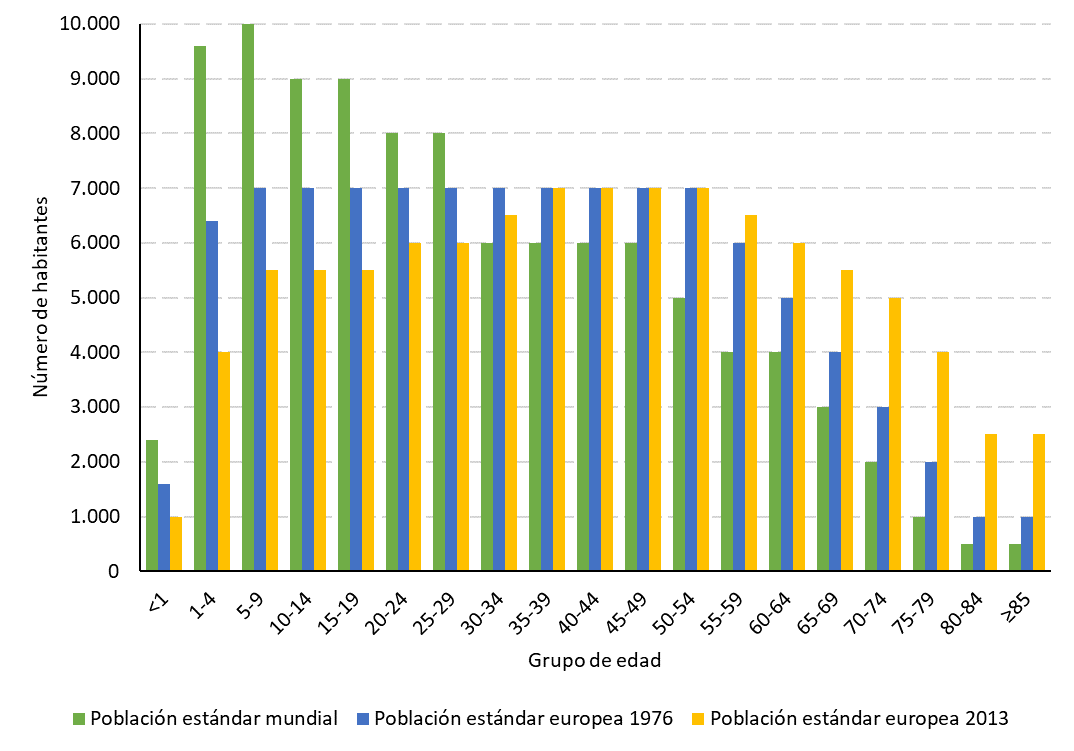
\includegraphics[width=\textwidth]{figuras/Figura4.png} \\

\newpage
\noindent \textbf{Tabla 1}. \textbf{Poblaciones estándar para el cálculo de tasas estandarizadas para 19 grupos de edad}.
\begin{table}[H]
	\begin{tabular}{lrrr}
		\hline
		Grupo de edad  &  \begin{tabular}[c]{@{}r@{}}Población estándar\\ mundial 1960\end{tabular}  &  \begin{tabular}[c]{@{}r@{}}Población estándar\\ europea 1976\end{tabular}   &  \begin{tabular}[c]{@{}r@{}}Población estándar\\ europea 2013\end{tabular} \\ \hline
		$<$1    &  2.400  &  1.600  &  1.000\\
		1-4      &  9.600  &  6.400  &  4.000\\
		5-9    &  10.000  &  7.000  &  5.500\\
		10-14   &  9.000  &  7.000  &  5.500\\
		15-19   &  9.000  &  7.000  &  5.500\\
		20-24   &  8.000  &  7.000  &  6.000\\
		25-29   &  8.000  &  7.000  &  6.000\\
		30-34   &  6.000  &  7.000  &  6.500\\
		35-39   &  6.000  &  7.000  &  7.000\\
		40-44   &  6.000  &  7.000  &  7.000\\
		45-49   &  6.000  &  7.000  &  7.000\\
		50-54   &  5.000  &  7.000  &  7.000\\
		55-59   &  4.000     &  6.000  &  6.500\\
		60-64   &  4.000     &  5.000  &  6.000\\
		65-69   &  3.000    &  4.000  &  5.500\\
		70-74   &  2.000     &  3.000  &  5.000\\
		75-79   &  1.000     &  2.000  &  4.000\\
		80-84   &   500       &  1.000  &  2.500\\
		$\geq$85  &  500  &  1.000  &  2.500\\ \hline
		Total  &  100.000  &  100.000  &  100.000\\ \hline
	\end{tabular}
\end{table}

\newpage

\noindent A continuación se muestra un ejemplo para el cálculo de tasas de incidencia: tasas brutas, específicas por edad y estandarizadas por edad.\\

\noindent \textbf{Ejemplo 1}. \textbf{Incidencia de cáncer de próstata en hombres. Provincia de Granada, 2013.}\\ Ejemplo de cálculo de tasas de incidencia: tasas específicas por edad (TEE), tasa bruta (TB) y tasa estandarizada por la población europea (ASR-E) tomando como referencia la población estándar europea de 1976 (PEE).

\begin{table}[H]
	\begin{tabular}{llrrrrr}
		\hline
		$i$ & \begin{tabular}[l]{@{}l@{}}Grupo\\ de edad\end{tabular}  & Población ($P_i$) & \begin{tabular}[c]{@{}r@{}}Número de\\ casos ($N_i$)\end{tabular}    &  $\text{TEE}_i$ &  $\text{PEE}_i$  &  $\text{TEE}_i* \text{PEE}_i$\\ \hline
		1 & $<$1 & 4.500 & 0  &  0  &  1.600  &  0\\
		2 & 1-4 & 20.075 & 0  &  0  &  6.400  &  0\\
		3 & 5-9 & 27.120 & 0  &  0  &  7.000  &  0\\
		4 & 10-14 & 25.726 & 0  &  0  &  7.000  &  0\\
		5 & 15-19 & 25.237 & 0  &  0  &  7.000  &  0\\
		6 & 20-24 & 28.262 & 0  &  0  &  7.000  &  0\\
		7 & 25-29 & 30.438 & 0  &  0  &  7.000  &  0\\
		8 & 30-34 & 36.044 & 0  &  0  &  7.000  &  0\\
		9 & 35-39 & 38.508 & 0  &  0  &  7.000  &  0\\
		10 & 40-44 & 36.546 & 0  &  0  &  7.000  &  0\\
		11 & 45-49 & 36.850 & 8  &  21,7  &    7.000  &  1,5\\
		12 & 50-54 & 32.594 & 17  &  52,2  &   7.000  &  3,7\\
		13 & 55-59 & 26.740 & 35  &  130,9  &  6.000  &  7,9\\
		14 & 60-64 & 21.895 & 67  &  306,0  &  5.000  &  15,3\\
		15 & 65-69 & 19.737 & 88  &  445,9  &  4.000  &  17,8\\
		16 & 70-74 & 15.123 & 92  &  608,3  &  3.000  &  18,3\\
		17 & 75-79 & 14.092 & 75  &  532,2  &  2.000  &  10,6\\
		18 & 80-84 & 10.671 & 47  &  440,4  &  1.000  &  4,4\\
		19 & $\geq$85 & 6.807 & 18  &  264,4  &  1.000  &  2,6\\  \hline
		& & & & & & ASR-E = 82,1\\ \hline		
	\end{tabular}
\end{table}
\vspace{-0.5cm}
\noindent Fuentes de información:
\begin{itemize}
	\item Registro de Cáncer de Granada. Número de casos de cáncer de próstata en la provincia de Granada, 2013.
	\item Instituto Nacional de Estadística. Población de hombres residentes en la provincia de Granada a 1 de Julio de 2013.
\end{itemize}

$$\text{TEE}_{14} = 100.000 * \dfrac{N_{14}}{P_{14}} = 100.000 *  \frac{67}{21.895}  = 306,0 $$ La tasa específica por edad para los hombres de 60 a 64 años es de 306 casos por 100.000 hombres.

$$\text{TB} = 100.000 * \sum_{i=1}^{19} \dfrac{N_i}{P_i} = 100.000 *  \frac{447}{456.965}  = 97,8 $$ La tasa bruta es de 97,8 casos por 100.000 hombres.

$$\text{ASR-E} = \sum_{i=1}^{19} \text{TEE}_i * \text{PEE}_i  = 82,1$$ La tasa estandarizada por la población europea es de 82,1 casos por 100.000 hombres. \\

\noindent \textbf{Otros indicadores}

\noindent Existen otros indicadores epidemiológicos que miden distintos aspectos de la incidencia, como las tasas truncadas, las tasas acumulativas, o las tendencias de la incidencia. Más información sobre estos indicadores puede encontrarse en el capítulo 9 de ``Registros de Cáncer: Principios y Métodos" (IARC) \cite{IARC1995}.

\section{Mortalidad}

Para la mortalidad, se pueden calcular de forma similar las mismas tasas que calculamos para la incidencia, cambiando el número de casos incidentes por el número de defunciones por cáncer.\\

Una defunción por cáncer se define como una muerte que es causada directamente por el cáncer, y no debe confundirse con defunciones de personas que tienen cáncer pero fallecen por otras causas (infarto, accidente de tráfico, ...).\\

A continuación se muestra un ejemplo para el cálculo de tasas de mortalidad: tasas brutas, específicas por edad y estandarizadas por edad.\\

\newpage
\noindent \textbf{Ejemplo 2}. \textbf{Mortalidad por cáncer de mama en mujeres. Provincia de Granada, 2013.}\\
Ejemplo de cálculo de tasas de mortalidad: tasas específicas por edad (TEE), tasa bruta (TB) y tasa estandarizada por la población europea (ASR-E) tomando como referencia la población estándar europea de 1976 (PEE).

\begin{table}[H]
	\begin{tabular}{llrrrrr}
		\hline
		$i$ & \begin{tabular}[l]{@{}l@{}}Grupo\\ de edad\end{tabular}     & Población ($P_i$) & \begin{tabular}[c]{@{}r@{}}Número de\\ defunciones ($D_i$)\end{tabular}    &  $\text{TEE}_i$ &  $\text{PEE}_i$  &  $\text{TEE}_i* \text{PEE}_i$\\ \hline
		1 & $<$1 & 4.149 & 0  &  0  &  1.600  &  0\\
		2 & 1-4 & 18.380 & 0  &  0  &  6.400  &  0\\
		3 & 5-9 & 25.345 & 0  &  0  &  7.000  &  0\\
		4 & 10-14 & 23.548 & 0  &  0  &  7.000  &  0\\
		5 & 15-19 & 23.674 & 0  &  0  &  7.000  &  0\\
		6 & 20-24 & 26.741 & 0  &  0  &  7.000  &  0\\
		7 & 25-29 & 29.494 & 0  &  0  &  7.000  &  0\\
		8 & 30-34 & 34.431 & 0  &  0  &  7.000  &  0\\
		9 & 35-39 & 36.199 & 4  &  11,1  &  7.000  &  0,8\\
		10 & 40-44 & 35.204 & 5  &  14,2  &  7.000  &  1,0\\
		11 & 45-49 & 36.540 & 6  &  16,4  &  7.000  &  1,1\\
		12 & 50-54 & 32.853 & 11  &  33,5  &  7.000  &  2,3\\
		13 & 55-59 & 27.334 & 19  &  69,5  &  6.000  &  4,2\\
		14 & 60-64 & 23.124 & 9  &  38,9  &  5.000  &  1,9\\
		15 & 65-69 & 21.835 & 8  &  36,6  &  4.000  &  1,5\\
		16 & 70-74 & 17.918 & 12  &  67,0  &  3.000  &  2,0\\
		17 & 75-79 & 18.563 & 12  &  64,6  &  2.000  &  1,3\\
		18 & 80-84 & 15.643 & 14  &  89,5  &  1.000  &  0,9\\
		19 & $\geq$ 85 & 12.954 & 23  &  177,6  &  1.000  &  1,8\\ \hline
				& & & & & & ASR-E = 18,8\\ \hline	
	\end{tabular}
\end{table}
\vspace{-0.5cm}
\noindent Fuentes de información:
\begin{itemize}
	\item Ministerio de Sanidad, Consumo y Bienestar Social. Número de defunciones por cáncer de mama en mujeres en la provincia de Granada, 2013.
	\item Instituto Nacional de Estadística. Población de mujeres residentes en la provincia de Granada a 1 de Julio de 2013.
\end{itemize}

$$\text{TEE}_{19} = 100.000 * \dfrac{N_{19}}{P_{19}} = 100.000 *  \frac{23}{12.954}  = 177,6 $$ La tasa específica por edad de mortalidad para las mujeres de 85 años o más es de 177,6 defunciones por 100.000 mujeres.

$$\text{TB} = 100.000 * \sum_{i=1}^{19} \dfrac{N_i}{P_i} = 100.000 *  \frac{123}{463.929}  = 26,5 $$ La tasa bruta de mortalidad es de 26,5 defunciones por 100.000 mujeres.

$$\text{ASR-E} = \sum_{i=1}^{19} \text{TEE}_i * \text{PEE}_i  = 18,8$$ La tasa de mortalidad estandarizada por la población europea es de 18,8 defunciones por 100.000 mujeres. \\

\section{Prevalencia}

\section{Supervivencia}